\newpage
\section{Results} \label{Results}

\begin{comment}
\textbf{How useful is Ampersand for designing registry systems by analysing public health legislation and regulations, in particular the \acrshort{big}.}
Hoe nuttig is Ampersand voor het ontwerpen van registratiesystemen door analyse van wet- en regelgeving op het gebied van volksgezondheid, in het bijzonder de Wet-BIG.

When investigating the research question, the following sub-questions will contribute to the answer to the research question.

Bij het onderzoeken van de onderzoeksvraag zullen de volgende deelvragen bijdragen aan het beantwoorden van de onderzoeksvraag. Gerelateerde vragen:
\end{comment}
\begin{wrapfigure}{r}{.5\textwidth} 
    
\includegraphics[scale=0.3]
        {Contented_Definitie_Ampersand_Wikipedia-1024x698.png}
    \caption{www.contented.nl/wat-weet-jij-van-het-en-teken-de-ampersand}
    \label{fig:Ampersand definition}
\end{wrapfigure}
The research focuses on the question of the usability of Ampersand(\&).
The ampersand sign~\footnote{\url{https://www.contented.nl/wat-weet-je-van-het-en-teken-de-ampersand}} and the Ampersand method both emphasize the meaning "and self-contained".
On the website of 
Ampersand~\footnote{\url{https://ampersandtarski.gitbook.io/documentation/why-ampersand/business-rules-in-ampersand}} 
we find an interpretation of the statement "standalone (op zichzelfstaand)".

During the graduation project, research was conducted into the suitability of Ampersand for designing registers for the government.
These registers are always based on legislation and regulations.
The research focuses on a specific law, namely the \acrshort{big}.

This law does not stand alone.
The associated laws and regulations are the following:
\begin{enumerate}
    \item Wet op de beroepen in de individuele gezondheidszorg
    \item Algemene wet bestuursrecht
    \item Besluit periodieke registratie Wet BIG
    \item Registratiebesluit BIG
    \item Tuchtrechtbesluit BIG
    \item Besluit gezondheidszorgpsycholoog
    \item Regeling periodieke registratie Wet BIG
    \item Regeling tarieven registratie beroepsbeoefenaren Wet BIG
    \item Algemene wet erkenning EU-beroepskwalificaties
    \item Besluit buitenslands gediplomeerden volksgezondheid
    \item Regeling erkenning EU-beroepskwalificaties beroepen in de individuele gezondheidszorg
\end{enumerate} 

In addition to the law-big, the investigation into the suitability of Ampersand also covers the above list of regulations.
Due to time-boxing it is not possible to analyze and process all associated laws and regulations.
The aim is not to provide a fully elaborated conceptual analysis, but to test Ampersand for usability.

The results of the study will be discussed in the following sections.
The research that focuses on the research question "\acrlong{research question}".
By answering the derived questions, we provide a view on the usability of Ampersand.





\begin{comment}
RQ1 - Welke kennis, in de rol van software engineer, is nodig om Ampersand te gebruiken.
[RQ1]- What knowledge, in the role of software engineer, is needed to use Ampersand.
\end{comment}
\def\rq{RQ1}

\begin{comment}
\textbf{How useful is Ampersand for designing registry systems by analysing public health legislation and regulations, in particular the \acrshort{big}.}

When investigating the research question, the following sub-questions will contribute to the answer to the research question.
\newline Related questions:
\begin{enumerate}
\item[RQ1]- What knowledge, in the role of software engineer, is needed to use Ampersand.
\item[RQ2]- What are the Concepts, Relationships and Rules in the \acrshort{big}.
\item[RQ3]- How are the laws and regulations set up so that they can be used in a useful way for the Ampersand method.
\item[RQ4]- What are the strengths and weaknesses (SWOT) in using Ampersand for registry systems for a government organization.
\end{enumerate}

Hoe bruikbaar is Ampersand voor het ontwerpen van registratiesystemen door analyse van wet- en regelgeving op het gebied van volksgezondheid, in het bijzonder de Wet-BIG.

Bij het onderzoeken van de onderzoeksvraag zullen de volgende deelvragen bijdragen aan het beantwoorden van de onderzoeksvraag. Gerelateerde vragen:
RQ1 - Welke kennis, in de rol van software engineer, is nodig om Ampersand te gebruiken.
RQ2 - Wat zijn de concepten, relaties en regels in de Wet-BIG.
RQ3 - Hoe zijn de wet- en regelgeving opgezet zodat ze kunnen worden gebruikt in een bruikbare manier voor de Ampersand-methode.
RQ4 - Wat zijn de sterke en zwakke punten (SWOT) bij het gebruik van Ampersand voor registratiesystemen voor een overheidsorganisatie.

\end{comment}



\subsection{Use of Ampersand}\label{use_of_ampersand}
When searching for the question "\acrlong{\rq}" it was decided to split this question even further and to label the items found.
A layout has been made in advance.
These items of this classification always provide a different perspective on the sub-question.
\begin{comment}
When asking questions about the knowledge required in the role of software engineers to be able to use Ampersand, the focus is not only on the Ampersand method itself.
We must also ask ourselves whether, in addition to Ampersand, knowledge of the underlying theory on which Ampersand is based is also required.
Is it necessary to know relationship algebra.
The environment in which a prototype runs also plays a role.
This includes browser settings and the use of containers (Docker) in which Ampersand runs.
During development we are dealing with an \acrfull{ide}.
The use of such a \acrshort{ide} for determining the usability of Ampersand is relevant.
Internet support is now indispensable when creating the scripts.
Scripting for Ampersand also requires support for web search capabilities.
But can this be found for a relatively unknown method like Ampersand?
Finally, we look at output produced by method.
Is it true that how the method is used also determines what comes out?
This applies to both the prototype and the generated documentation.
Subsequently, the approach to this process, the use of the method, among other things, determines the result.
These aspects will be discussed in the following paragraphs.
The sub-questions can be further subdivided into small parts.
Starting from the question "\acrlong{rq1}", the question then follows which observations relate to this knowledge.
Is it knowledge about only Ampersand or is knowledge also required of relation algebra.
By working with Ampersand, we are also confronted with the environment in which we develop it.
Ampersand stands alone as a language, but in use there are development tools like \acrlong{vsc} in this case.
To run it, you need a Docker container.
That is at least the implementation as the \acrlong{ou} provides.
During the development phase, examples are searched on the internet.
And these are generally easy to find, is that also the case at Ampersand?
Ampersand also provides documentation and a prototype.
Here too, knowledge of Ampersand is required.
Finally, you also have to ask yourself whether the way Ampersand is used, the approach to the project, also requires knowledge of Ampersand.
There are a number of angles that play around Ampersand's knowledge.
\end{comment}

\subsubsection{Observation summary}
A list of occurrences is included at the end of this section.

The Ampersand item has a wide palette of comments.
This is about the setup of the tool, looking for examples to be able to work with it.
Considerable experience is required to work with it.
A remark that comes up a lot with various items is about overview.
Overview in terms of usage and how to track progress.

\subsubsection{Observations }
The observations in order of multiplicity of occurrence within \acrshort{\rq}.
\newcounter{subsubsubsection}[subsubsection]
%Concept:
%- notatie 2
%- shared concepts 2
%- werkwijze bij het ontdekken van een concept
%- bepaalde concepten als datum en tijd zijn complex in gebruik
%- waar worden bepaalde concepten gebruikt (in script) en in relaties
%- dezelfde concepten zijn vaker te definieren, onbewust zou dit redefines kunnen worden 2
%- wanneer is iets een concept -> immutable
%v
\parlabel{Concept}
The term Concept is an important concept within Ampersand.
The Concept is described in detail on the website of Ampersand~\footnote{\url{https://ampersandtarski.gitbook.io/documentation/the-language-ampersand/syntactical-conventions/the-concept-statement}}.
However, there are observations on the Concept that are described on this site.
These are observations related to the notation of a Concept.
The fact that a Concept is immutable is also described there.
An example of the use of the concept of date is also described.

%v
The comments regarding items not mentioned on the website relate to the use of the Concepts.
It concerns the use and reuse of concepts within the scripts.
The definitions of concepts go beyond the patterns.
It is possible to use the same Concepts in multiple places.
Redefinition of a Concept is possible with impunity.
This redefinition may lead to the same Concept with a different definition.

\parlabel{Interface, CRUD}
% CRUD met hoofd en kleine letters
% de concepts in de interface moeten van het type object zijn
% op de crud U/l wordt niet gecontroleerd wijzigingen hebben niet altijd inpact
% max 1 TOT in de interface, anders wordt de data niet opgeslagen
% waarneming interface behoort tot design en niet enkel prototype
% views in HTML niet werkend te krijgen
% linkto in de interface; dropdown, signatuur
% browser issue omdat de cache vasthoud
% target blank wordt verwijderd.
The interface has some implementation challenges.
The website of the Ampersand refers to the operation of the Interface from several places.
Within the Ampersand notation it falls into the Service category.
The \acrlong{crud} usage leads to confusion.
The use of upper and lower case letters is not validated.
And in some situations it has no visible effect either.

When setting up the Interface, the requirement is that the Input Concept is of type object.
\begin{lstlisting}
INTERFACE RegistratieArts FOR MEDEWERKER : I[Registratie] cRud
\end{lstlisting}

The use of the Interface within the browser has as a point of interest that the browser has a cache that stores outdated data.
It is necessary to clear the cache after changes in the Interface.

The multiplicity of total \footnote{For any a in A there must be at least one b in B in the population of r} must be only one in the Interface.
With multiple occurrences in one Interface, the data can no longer be stored.

A LINKTO signature occurring in multiple Interfaces causes unwanted behavior in the Interface.
When clicking on the link, a choice is offered of all links with the relevant signature.

The use of Views within the Interface is well described in the documentation, but not clear enough.
It is not always working.
The examples do not contribute to this either.

The Interface is part of the design.
It was expected that this would only be part of the prototype, but is of course part of the whole.

Bij de interface wordt een \acrfull{crud} per Concept en Relatie opgegeven.
Hierbij is de hoofdletter voor de uitvoering van de methode en de lowercase het niet uitvoeren van de methode.
Niet in alle gevallen geeft het  omzetten van lowercase naar uppercase een verandering in het gedrag.


\parlabel{Ampersand}
% the documentation gives an indication of how to configure ampersand and make it work locally. Using XAMP.  All this is not going to work.     Not clear why.     It did work in a Docker environment.
% Little to be found about Ampersand except in its own repos
% The need for overview is there as the script grows.
% it comes down to wanting to maintain an overview.     That is what I want with the annotation.
% Quick fix of a bug in Ampersand by the development team.
% There should always be someone with experience in the background or in the collaboration.
% Practice a lot and keep using it.
Implementing Ampersand locally does not work.
Despite description about the possible use of XAMPP.
It is possible, with some help, to make this work via Docker.

Not much information is available on the internet about Ampersand outside of the Ampersand website itself.
In addition, stackoverflow is a resource and information can be found on GitHub\footnote{\url{https://github.com/AmpersandTarski}}.

When processing the \acrshort{big} in Ampersand it is difficult to keep an overview.
Overview from different perspectives.
Pick up where you left off in the text.
And which parts are defined as concept and relationship.
The latter to avoid duplicates.

\parlabel{Rule}
%To implement rules, knowledge of Ampersand is required and many examples must be used.
% You are not forced to work in any particular structure.
% add a ROLE with a MAINTAINS
% Many messages remain open if not all \A{rule}s are met
%     This is quite a steep learning curve.
% create delete rules 
% If there is an automatic \A{rule}, should there still be a validation rule on it?
Some of the comments are about the learning curve of the rules.
It is not obvious how the rules work.
Lots of examples and explanations are needed to get it working.

It is also mandatory to use a ROLE in combination with the Rule.
This is necessary to indicate which role the rule may use.
\begin{lstlisting} [caption=Persoon.adl, numbers=none]
       ---- relaties
        RELATION naam [Persoon*Naam][UNI,TOT,SUR]
            PRAGMA "De persoon met het id " " wordt " " genoemd."
            MEANING "Elke ingeschrevene moet een naam hebben en een naam kan bij meerdere personen behoren."
            POPULATION naam [Persoon*Naam] CONTAINS 
            [ 
                ("P001", "Edelaar"),
                ("P002", "Jansen"),
                ("P003", "Pietersen") ]
        --IDENT "Persoon" : Persoon(naam[Persoon*Naam])
        ROLE USER MAINTAINS TotNaam
        RULE TotNaam : I[Persoon]  |-  naam[Persoon*Naam];naam[Persoon*Naam]~
            MEANING "meaning"
            MESSAGE "Er moet een naam ingevuld worden."
            VIOLATION ( TXT "Voor persoon ", SRC I , TXT " is geen naam ingevuld.")
\end{lstlisting}

A rule cannot be met, so the data element cannot be validated.
In that case, messages will return.
When it is used as an API, a message is returned for each element that is not validated.
With the prototype, it is possible that the screen is filled with notifications.
There are also notifications from other inputs, these keep coming back in the relevant screen.

Rules can be used to add data automatically.
The question that this raises is whether it is still necessary to add a validation rule.

\parlabel{Conceptual analysis} 
%  Formatting in Ampersand (\A{pattern}s) has consequences for the \A{Conceptual analysis}.
%     First the definition is shown, then the name of the relation and below that the meaning again. The layout of the Conceptual design doesn't seem quite logical and is therefore confusing.
% Break enters in the \acrshort{ide} also produce extra newlines in the output.    This causes the formatting to go wrong.
% }: The "disclaimer" does not appear in the Conceptual analysis.
% when generating a \A{Conceptual analysis} the doc gets the name of the first concept.
% The starting point is to make the Conceptual analysis in Dutch.
% Discussing the \A{Conceptual analysis} should be done theme by theme.
The observations regarding the Conceptual analysis mainly relate to the formatting of the output.
The order of the information presented is not entirely logical.
The following is noted in the script.
\begin{lstlisting} [caption=Persoon.adl script with CONCEPT Voornaam, numbers=none]
        --voornaam
        CONCEPT Voornaam "Alle voornamen van de Persoon zoals dit is vastgelegd binnen de BRP."
            REPRESENT Voornaam TYPE ALPHANUMERIC
            PURPOSE CONCEPT Voornaam
                {+
                In artikel 3 lid 2 is aangegeven dat de voorna(a)m(en) een onderdeel is/zijn van de identificatie van de zorgverlener.
                +}
\end{lstlisting}
\begin{tcolorbox} [title=Conceptual analysis "Definitie Voornaam"]
In artikel 3 lid 2 is aangegeven dat de voorna(a)m(en) een onderdeel is/zijn van de identificatie van de zorgverlener.\\
\\
\textbf{Definitie Voornaam:}\\
   Alle voornamen van de Persoon zoals dit is vastgelegd binnen de BRP.
\end{tcolorbox}

Where the meaning is placed above the headline and the definition below.
This was initially confusing because it was not immediately clear that the above meaning belonged to the definition.

Strange behavior was that the name of the document turned out to be the name of the first Concept mentioned.

Since the law is in Dutch, the analysis is also in Dutch.
It is remarkable that the Dutch language is supported together with English.
Not much international exposure.

The discussion of the analysis is done theme by theme, i.e. pattern by pattern.
This is to scope the discussion with the user.

\parlabel{Relation}
%: Each \A{relation} is part of a record structure. Good to discover how the database structure is established.     It is probably stated somewhere how this happens.     But this can be determined through reversed engineering.     Above all, it provides insight and makes it more tangible.
%     Only the first position is uppercase or lowercase.
% An \A{relation} that is univalent is a function.    A one function there can only come out one thing.
% : Immediately add the description when recording 
% There is no find able relationship
% A \A{concept} and a \A{relation} can be defined several times within your own patterns.
From a technical point of view, a relationship is part of the record structure.
An example is the Concept Voornaam with a relation, named \mbox{voornaam}.

\begin{lstlisting} [caption=Persoon.adl script with RELATION voornaam, numbers=none]
        RELATION voornaam [Persoon*Voornaam][UNI]
\end{lstlisting}
In combination with the multiplicity UNI, this is included as a separate table shown in figure~\ref{Fig:voornaam-in-persoon} and as an attribute in the table Persoon in figure~\ref{Fig:voornaam-in-persoon}.
\begin{figure}[!htb]
   \begin{minipage}{0.48\textwidth}
       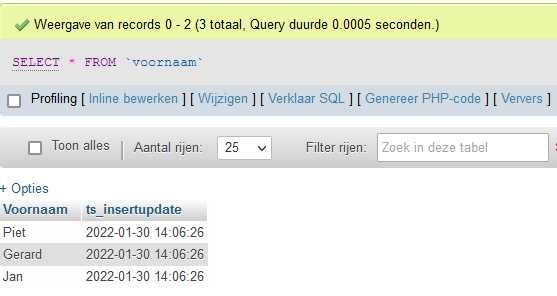
\includegraphics[width=.6\linewidth]{phpMyAdmin_Voornaam.png}
       \caption{Concept Voornaam}\label{concept-voornaam}
   \end{minipage}\hfill
   \begin{minipage}{0.48\textwidth}
       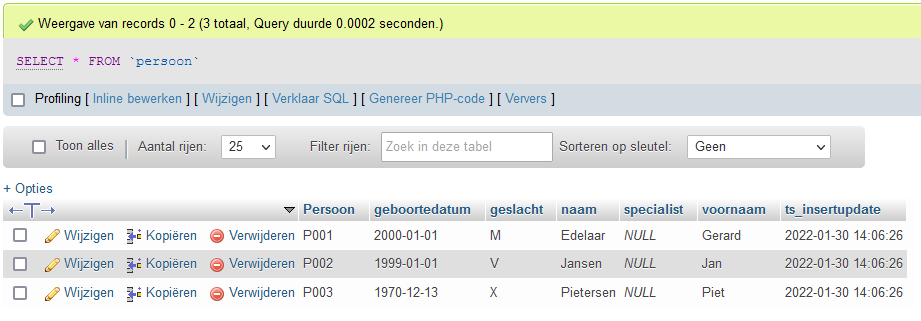
\includegraphics[width=.9\linewidth]{phpMyAdmin_Persoon.png}
       \caption{Relatie voornaam in Persoon}\label{Fig:voornaam-in-persoon}
   \end{minipage}
\end{figure}

\begin{wrapfigure}{l}{0.2\textwidth}
    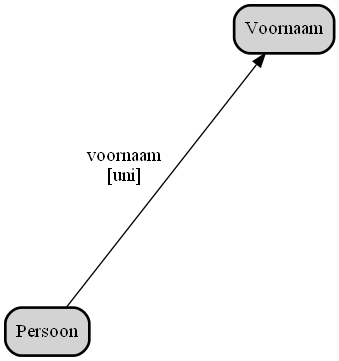
\includegraphics[width=0.9\linewidth]{CDConceptVoornaam.png} 
    \caption{\label{fig:CDConceptVoornaam}CDConceptVoornaam}
\end{wrapfigure}
Conceptually, this is modeled in this way, figure~\ref{fig:CDConceptVoornaam}.
This shows that from the Concept Person there is a \acrlong{uni} relation to the Concept Voornaam.
In data modeling terms, this is called a 1:n Persoon to Voornaam relationship.

\begin{wrapfigure}{l}{0.65\textwidth}
    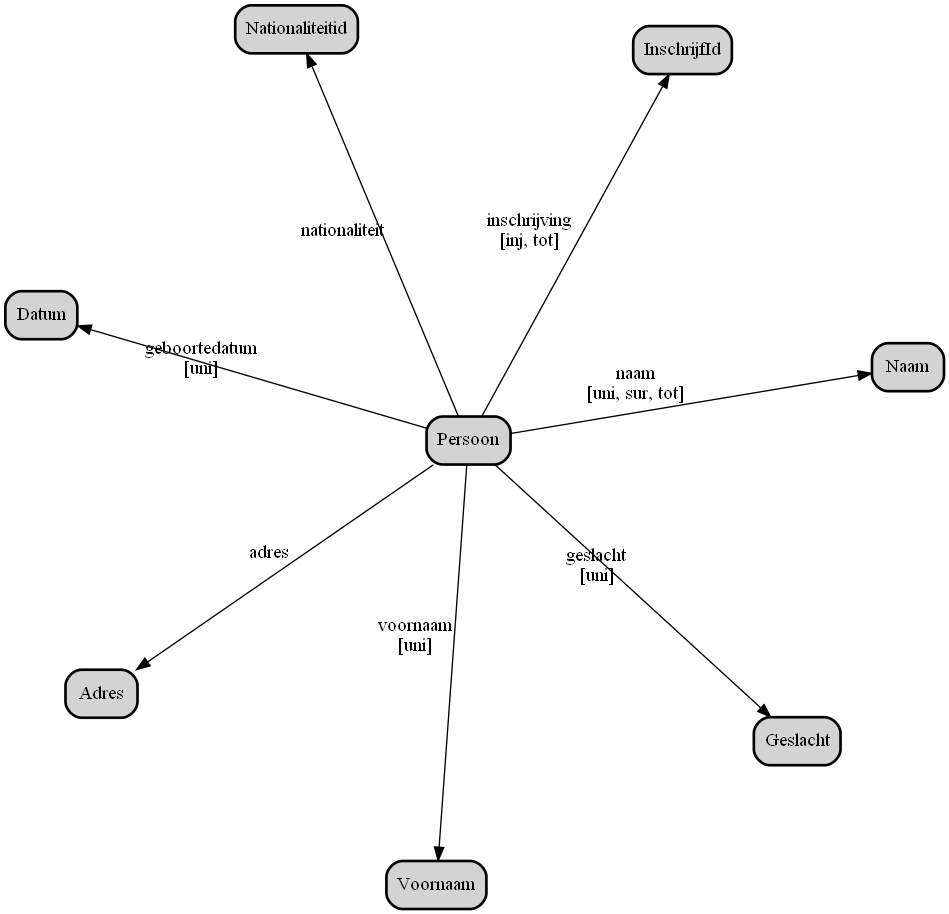
\includegraphics[width=0.9\linewidth]{CDConceptPersoon.png} 
    \caption{\label{fig:CDConceptPersoon}CDConceptPersoon.}
\end{wrapfigure}
In addition to the relation with \mbox{Voornaam}, several relations can be recognized on the Concept \mbox{Persoon}, see figure~\ref{fig:CDConceptPersoon}.
These have different multiples.
The relation of \mbox{Persoon} to \mbox{Geslacht}, \mbox{Voornaam} and \mbox{Datum} are of the type \acrlong{uni}.
From \mbox{Persoon} to \mbox{InschrijfId} is of type \acrlong{inj} and \acrlong{tot}.
The relation \mbox{Persoon} to \mbox{Naam} is of type \acrlong{uni}, \acrlong{sur} and \acrlong{tot}.

There are also relationships that do not have multiplicity.
Such as the concepts of \mbox{Nationaliteit} and \mbox{Adres}.  
The lack of multiplicity means that this is an n:m relationship.
In the phpMyAdmin admin console, we see this as multiple tables.

If we look at the \mbox{Nationaliteit} Concept, we see in the admin console~\footnote{PhpMyAdmin} that three tables related to Nationaliteit have been created.
These are the tables \mbox{nationaliteitId}, \mbox{nationaliteit1} and \mbox{nationaliteit2}.
There is no conceptual overview in which these three entities return.
Also the technical model gives no indication of the existence of \mbox{nationaliteit2}.
The other two entities do appear in the technical model.
The entities \mbox{nationaliteitId} and \mbox{nationaliteit2} have a 1:1 relationship.
Caused by a adding of a technical field named Id.
This is probably the reason that they are not explicitly included.
The relationship between \mbox{nationaliteitId} and \mbox{nationaliteit1} is of type 1:n.

As we also see with the Concept, it is also possible for relations to specify the same relation name with a different meaning.
This can be seen in the document, but is not immediately noticed in the scripts.

The definition and also when filling in the meaning nothing is enforced.
Any description is good.
Good practice is also missing.

When creating the scripts, it is good practice that the designer also establishes a definition and meaning immediately after creating the relationship.
However, this usage is easily overlooked when enthusing and testing the scripts.

\parlabel{Api}
% No swagger is created for the \A{api};
% Postman works with api/v1/resource
% Using Postman, the \A{api} features were tested.
% return values 
% A change in the back-end, so an Ampersand change, then the front end almost certainly has to change with it.
To use the API properly, it is necessary to know the schema.
Usually this is included in Swagger.
This one is now missed.

The APIs are looked up in the log lines and then tested via Postman.
And that works well.

A disadvantage of working with APIs is that the backend returns the message included in the validation.
It is common to get a return code here.

\parlabel{Pattern}
% isolation  pattern, lukte niet
% patterns = subsystemen
% gebruik van definitie
% subsystemen vooraf bepaald.
A Pattern within Ampersand has the level of subsystem.
A pattern is a set of rules that describes a theme or a general reusable solution to a commonly occurring problem~\footnote{\url{https://ampersandtarski.gitbook.io/documentation/the-language-ampersand/patterns\#purpose }}
Within the \acrshort{big} several registers can be identified.
A register is housed in a pattern.
Attempted to deploy the registry in isolation.
This did not work, because Ampersand does not support multi context.

Because a pattern has the level of a subsystem, an attempt was made to classify it beforehand.
That did not work, in this case.
It is better to let it arise.

\parlabel{Documentation}
% browser issues bij doc in html
% persistent lnks 
% docu in verschillende outputs wijze
% met het werken vergeten te documentern
When generating the documentation, it is noticeable that in addition to the multitude of documentation, there is also the possibility of different output type options.
When executing in HTML it was noticed that the images in the Firefox browser were not shown.

When experimenting with extra html headers within the definition, the meaning and the purpose.
However, this does not always yield the desired result.
Adding <H1> header causes the new chapters to be inserted.

\parlabel{Include}
% refactoring nodig, verwijderde include pas gemerkt bij error
% includes stuurt docu
% include zijn niet altijd nodig, in de root is voldoende
% include bevorderd herbruikbaarheid
Removing an include is not noticed until compilation.
The tool in which Ampersand script is developed does not include refactoring capability.

Includes are mainly used to send documentation.
The scripts usually find out on their own when an include is needed for compilation

Small modules promote reusability.


\parlabel{Multiplicity}
% 1 TOT per interface
% excel files toont data structuur
% uitshrijven mu
% excel gebruiken voor mu
To make use of multiplicity, there are two things that can be done.
First, make a description of multiplicity.

\begin{tabular}{ || l | l | l ||}
    \hline
    UNI & P->0-1 H &  most\\  \hline    
    TOT & P->1-* H  & least\\  \hline
    INJ & H->1 P  &   one\\  \hline
    SUR & H->1-* P &  at least 1\\ \hline
    \end{tabular}
    
In addition, use an excel sheet in which the relationships are provided with a multiplicity.
This gives insight into the shape of the relationships.

\parlabel{Docker}
% steeds nieuwe directories in RAP
% learning thing
% isolation niet mogelijk ivm multicontext
Using the RAP~\citeNonPub{michels_development_2015} within Docker produces undesirable behavior because new directories are always created with each modification.
As a result, it is not clear where the sources are.
Also, includes cannot be used at that time.

The attempt to isolate each registry and run as a separate instance fails due to the issue of multicontext.
A generic part is always reused within the registers, but with overlapping of the shared data.

In addition to Ampersand, it is also necessary to have basic knowledge of Docker.

\parlabel{Prototype}
% start niet in localhost
% postman koppeling werkt
% test scenario's
The documentation hints at a local installation using XAMPP using its own stack.
However, this is not working.
Finally switched to a local Docker implementation with help, which worked fine.

To test the APIs of the prototype, an instance of Postman~\footnote{\url{https://www.postman.com/}} was installed to experience whether the prototype could also be used externally.
And this worked well.

Ampersand does not provide any testing options.
This could be arranged via Postman, but then only APIs are tested.
Otherwise, a Selenium tool could be used to further test the prototype.

\parlabel{Register}
% multicontext
In order to be able to run registers independently of each other, the generic software part and the shared data part must be able to be implemented.
This is not possible because the implementation of the shared part cannot be installed separately.
Each separate installation overwrites the previous one.
As a result, it can only be implemented as a whole.

\parlabel{Visual Studio}
% refactoring
% Ampersand extension die hangt
% latex support
The use of \acrfull{vsc} is recommended because an Ampersand extension has also been developed.
Possibly due to issues on your own system, this extension did not work properly.
No more issues were encountered later in the process.

Using \acrshort{vsc} does cause issues when refactoring the scripts.
Except for a standard search and replace, no support is offered with refactoring.
The consequences of this are experienced at compile time.

An extension of \acrshort{vsc} is handling Latex text.
Besides being necessary for this document, there is also an option to generate the Conceptual analysis in Latex.
However, the delivered result must first be processed before it can be used.
Working with Latex within \acrshort{vsc} is not nice working.
Processes are started in the background that eventually hang up the entire PC.

\parlabel{Php}
% maken van php functies kan wel, maar is niet duidelijk hoe
% zijn sommige zaken niet beter af in andere talen of tools
It is possible to add functions written in PHP.
However, it is not clear how this should be done now.

There are topics that lend themselves better as an external function than as part of Ampersand.
In the elaboration, a guid is defined as a Big number.
Such a number is not suitable to be exposed.
Ampersand does not lend itself to building a routine that generates a readable big number.

\parlabel{Represent}
% onverwacht gedrag door represent statement
% datetime represent kan niet geconverteerd worden naar excel
By using the Represent statement, the interface reacts differently.
It is unclear why that happens.
By giving a Concept a Represent option, the prototype will suppress an add option.
Where previously there was a "+" as an add-on option, this option will disappear when using the Respresent.
It is not clear whether this is desirable or undesirable behaviour.

Using the DATETIME Represent option and exporting the populations to Excel ensures that this concept is not carried over to excel.
The conversion to Excel stops at this point.

\parlabel{PDF, RTF, XML and JSON}
When processing text, it is a challenge to keep track of what has been processed and what has not yet.
The text does not always run sequentially during processing.
In order to keep track of what has been processed, a possibility has been sought to do this.
The input texts can be processed in various formats.
In HTML format, downloaded or online.
The PDF format provides the ability to highlight text and add annotations.
The same can be done with RTF, but in a text editor.
Via XML and JSON tags or elements could be added that could be read out and processed into a script by means of a program that has yet to be written.
The latter is a project in itself and at first sight it is a lot of work.
And the question is whether this will yield results.
The latter especially in the control phase.

\parlabel{Other}
% Ampersand moet in de architectuur passen of architectuur moet aangepast worden
% CRUD toepassing 
% flexibiliteit A in gebruik en aanpassing
% lifeccyle zit niet echt in de wet, maar moet wel 
% linkto -> gedrag van 
% Obsedian
% RAP
% validation -> inzetbaarheid A
The use of Ampersand within an organization is not only the use of the tool and the method.
What also plays a role is the usability within the existing architecture.
Or the willingness to adapt the architecture to the use of Ampersand.

Ampersand is very flexible in use.
The Concepts and Relations are easy to realize.
Adjustments and extensions are easy to make.

What must be taken into account is the lifecycle of data.
That's not typically an Ampersand issue.
The description of the law is not such that it provides clarity in, for example, making registers and also cleaning them up.
In short, lifecycle thinking is not so much in legislation and regulations.

One of the important features of Ampersand is doing the validations.
Validations are enforced by the Rules and Relations.
This can be experienced in practice through the prototype and the use of APIs.

Using a Linkto with the same signature of the relationships produces unexpected interface behavior.
By the same signature, the Linktos on the relations are all shown and it is, as far as I know, not possible to specify the desired link.

\newpage







\begin{comment}
RQ2 - Wat zijn de concepten, relaties en regels in de Wet-BIG.
[RQ2]- What are the Concepts, Relationships and Rules in the \acrshort{big}.
\end{comment}



\subsection{Ampersand Conceptual Analysis}
[RQ2]- What are the Concepts, Relationships and Rules in the \acrshort{big}.


\begin{comment}
RQ3 - Hoe zijn de wet- en regelgeving opgezet zodat ze kunnen worden gebruikt in een bruikbare manier voor de Ampersand-methode.
[RQ3]- How are the laws and regulations set up so that they can be used in a useful way for the Ampersand method.
\end{comment}
\def\rq{rq3}
\cntA{Ampersand}
\cntA{api}
\cntA{classify}      
\cntA{concept}   
\cntA{Conceptual analysis}
\cntA{concepten}     
\cntA{crud}           
\cntA{Docker}   
\cntA{documentation}
\cntA{flexible}     
\cntA{include}
\cntA{interface}     
\cntA{latex}
\cntA{Lifecycle}
\cntA{linkto}        
\cntA{multiplicity}  
\cntA{Obsidian}
\cntA{pattern}
\cntA{php}
\cntA{population}    
\cntA{prototype}
\cntA{RAP}            
\cntA{relation}
\cntA{represent}      
\cntA{rule}
\cntA{VSC}
\cntA{XML}
\cntA{JSON}
\cntA{RTF}
\cntA{PDF}
\cntA{validation}
\cntA{architecture}



\begin{comment}
RQ3 - Hoe zijn de wet- en regelgeving opgezet zodat ze kunnen worden gebruikt in een bruikbare manier voor de Ampersand-methode.
\end{comment}
\subsection{The wet BIG and Ampersand}
[RQ3]- How are the laws and regulations set up so that they can be used in a useful way for the Ampersand method.
\begin{enumerate}
    \item rq3-2 door het lezen van de wet wordt er een opbouw duidelijk -> persoon; inschrijving; registratie->beheer; tucht->maatregelen; 
    \newline\textbf{obs}: de hoofdlijnen van de wet lijken, voor een niet jurist, duidelijk

    \item rq3-3 12-9 er zijn delen van de wet die niet meer geldig zijn, deze worden niet meegenomen
    \newline\textbf{obs}: de wet is best complex opgebouwd, en het mogelijk om terug te gaan in de tijd.
    Keuze die gemaakt is, is om niet terug te gaan in de tijd.
    
    \item rq3-4 12-9 er zijn meer wetten bij betrokken dan enkel de wet BIG
    \newline rq3-6 12-9 naast de web zijn ook besluiten van belang
    \newline\textbf{obs}: op de website van de wet zijn verwijzingen opgenomen naar andere wetten en regelgeving.
    
    \item rq3-5 12-9 jurisprudentie buiten scope -> nagaan of dit wel het geval is. 
    Maar beargumenteren waarom dit niet in een informatie systeem opgenomen zou moeten worden.
    \newline\textbf{obs}: is geen observatie maar een mening !!!

    \item rq3-7 het toevoegen van de juiste beschrijving bij een concept en relatie is nog niet zo eenvoudig; gemakkelijk om af te dwalen en een eigen interpretatie toe te voegen. 
    Ontbreekt een directe toets.
    \newline\textbf{obs}: tijdens het opstellen van concepten en relaties moet er direct een beschrijving bij van de positie waar het element vandaan komt.
    Dit gebeurt niet altijd omdat de scripttaal je zodanig bezig houdt (veel gepruts) zodat er vergeten wordt om de tekst toe te voegen.
    
    \item rq3-8:19-9: stelling in de wet dat er meerdere registers zijn. 
    Er is een register per beroepsgroep. 
    Mogelijk moet de indeling van de scripts ook op die wijze plaatsvinden.
    \newline\textbf{obs}: in de tekst van de wet wordt gesproken over meerdere registers. 
    De huidige implementatie Zorro laat zien dat er maar één register is geimplementeerd, met verschillende workflows voor de afhandeling van de beroepen (de feitelijke registers).
    
    \item rq3-9:19-9: opbouw van de registers is gelijk, registratie wordt ook wel inschrijving genoemd
    \newline\textbf{obs}: geen
    
    \item rq3-10:12-10: opmaak van de naam staat niet in de wet letterlijk genoemd, maar moet conform GBA/BRP normen. waar staat dat dan?
     \newline\textbf{obs}: is het relevant dat dit er niet in staat. 
     Dit zou op een andere plaats van in Ampersand afgedwongen kunnen worden. 
     Input validaties
     
    \item RQ3-11:12-10: zaken als autorisatie besluiten waardoor een informatie systeem BRP gegevens mag ophalen kom je in de wet niet tegen.
     \newline\textbf{obs}: de wet is niet gericht op de vertaling naar ICT
     
    \item rq3-12:12-10: ook kom je zaken als de termijnenwet niet tegen.
     \newline\textbf{obs}: geen
     
    \item rq3-13:17-10: in wetbig is geen lijst specialismen opgenomen, waar dan wel
     \newline\textbf{obs}: in de wet wordt wel verwezen naar specialisme
     
    \item rq3-14:19-10: een persoon en een big-nummer zijn heel verschillende zaken. Persoon is immutable, big nummer niet. Ze hebben wel een relatie met elkaar.
     \newline\textbf{obs}: in het spraak gebruik worden deze nog wel eens door elkaar gebruikt. 
     zodat het lijkt dat een persoon equivalent is aan een bignummer
     
    \item rq3-15:24-10: in de wet wordt de nationaliteit genoemd, ook wordt gerefereerd aan de EU en niet-eu bewoners, maar er wordt niet onderkent dat de nationaliteit definitie per land wordt gedefineerd.
     \newline\textbf{obs}: beperking van de wet
     
    \item rq3-16:24-10: voor nederland geldt dat we een landentabel hebben van de Rvig. Dit zijn nationaal vastgestelde en onderhouden tabellen. Er is hier dan ook geen onderhoudsfunctie op nodig.
     \newline\textbf{obs}: er is meer dan de wet
     
    \item rq2-17:10-11: een nl persoon heeft een adres dat aan de opmaak van de BRP moet/kan voldoen (zou een standaard bouwblok voor moeten zijn!), een buitenlands adres is onduidelijk wat hiermee moet.    
     \newline\textbf{obs}: zie rq-10
\end{enumerate}

\subsubsection{Reading law}
\begin{comment}
Hoort dit niet bij rq3?
plaats hier de afgehandelde items.
\end{comment}
\begin{enumerate}
    \item rq1-23:24-10: \textbf{wet} lezen is een vak 
    \newline\textbf{obs}: zie item
    
    \item rq1-25:12-9: eerst \textbf{overzicht} maken van de alle wetten en regelingen
    \newline\textbf{obs}: scoping belangrijk
    
    \item rq1-26:12-9: ook de wetten en de regelgevingen kunnen nog weer \textbf{verwijzigen} hebben naar andere wetten en regelgevingen. Omdat ze daarop gebaseerd kunnen zijn of deze uitbreiden.
    \newline\textbf{obs}: dat is waar.
    
    \item rq1-27:12-9: er zijn ook wetten en regels die niet opgenomen zijn in deze specifieke wet, maar geldig zijn vanuit een hoger liggende wet (implicite \textbf{verwijzingen}). 
    Denk hierbij aan de grondwet. 
    In geval van big zou dit bv de archiefwet kunnen zijn of de termijnenwet en strafrecht.
    \newline\textbf{obs}: hoe komt je tot een volledig overzicht van wetten en regelgeving
    
    \item rq1-28:12-9: regelgeving over een afgesloten en verleden, wordt niet meer meegenomen. 
    Deze is niet meer geldig. 
    Doel is niet om historie op te bouwen maar de huidige wet te ondersteunen.
    \newline\textbf{obs}: geen observatie maar meer scoping
    
    \item rq1-29:12-9: Niet alle wet- en regelgeving mbv BIG vinden we terug onder de \textbf{zoekterm} big.
    \newline\textbf{obs}: je moet er attend op zijn dat er meer is dan enkel BIG
    
    \item rq1-42:21-10: het is makkelijk om van de wetsteksten af te wijken. 
    Juist omdat deze zo lastig te lezen zijn. 
    En enigszins \textbf{kennis van de wet}cq het proces maakt dat eigen interpretatie snel gemaakt is. 
    Action research maakt ook dat je snel in deze valkuil stapt.
    \newline\textbf{obs}: zie item
    
    \item rq1-61:9-11: er zou een check op geb datum moeten komen(\textbf{rule}), dat iemand minimaal 18 moet zijn. 
    Klinkt logisch, maar is een afgeleide regel. 
    dus niet opnemen. 
    Deze zit al impliciet in de opleidingseis. 
    De duur van de opleiding maakt al dat iemand minimaal 18 jaar is voor dat de opleiding is afgerond.
    \newline\textbf{obs}: zie item
    
    \item rq1-95:29-12: de opmaak van een \textbf{concept} bignummer  is niet de wet opgenomen
    \newline\textbf{obs}: zouden er eisen zijn aan het bignummer nu is het volgens mij 8 cijfers, maar zou dit ook zo moeten zijn. 
    Een guid is misschien vanuit gebruikersvriendleijkheid niet zo handig
\end{enumerate}


\begin{tabular}{ || l | c | c ||}
    \hline
    object in \rq & count & y\\
    \hline\hline
    \tabifA{Ampersand}
    \tabifA{architecture}
    \tabifA{api}
    \tabifA{classify}      
    \tabifA{concept}     
    \tabifA{Conceptual analysis}
    \tabifA{crud}           
    \tabifA{Docker}   
    \tabifA{documentation}
    \tabifA{flexible}    
    \tabifA{include}
    \tabifA{interface}     
    \tabifA{JSON}
    \tabifA{latex}    
    \tabifA{Lifecycle}
    \tabifA{linkto}        
    \tabifA{multiplicity}  
    \tabifA{Obsidian}
    \tabifA{pattern}
    \tabifA{PDF}
    \tabifA{php}
    \tabifA{population}    
    \tabifA{prototype}
    \tabifA{RAP}            
    \tabifA{relation}
    \tabifA{represent}      
    \tabifA{RTF}
    \tabifA{rule}
    \tabifA{validation}
    \tabifA{VSC}
    \tabifA{XML}

\end{tabular}

\newpage


\begin{comment}
RQ4 - Wat zijn de sterke en zwakke punten (SWOT) bij het gebruik van Ampersand voor registratiesystemen voor een overheidsorganisatie.
[RQ4]- What are the strengths and weaknesses (SWOT) in using Ampersand for registry systems for a government organization.
\end{comment}
\begin{comment}
RQ4 - Wat zijn de sterke en zwakke punten (SWOT) bij het gebruik van Ampersand voor registratiesystemen voor een overheidsorganisatie.
\end{comment}

\subsection{Ampersand in government environment}
[RQ4]- What are the strengths and weaknesses (SWOT) in using Ampersand for registry systems for a government organization.
\begin{enumerate}
    \item rq4-1 A kan niet rekenen; Maar aangezien A statisch is, kunnen proces gegevens op andere manier worden bewaakt.
    \newline\textbf{obs}: kan niet rekenen!
    
    \item rq4-2 api koppeling werkt goed, echter komen hele meldingen terug; zouden eigenlijk codes moeten krijgen 
    \newline\textbf{obs}: api returned een tekst/melding -> daar kunnen aanroepende applicaties meestal niet zo goed mee overweg. 
    gebruikelijk is om een code en soms met tekst terug te geven. 
    denk hierbij aan httpresponse codes
    
    \item rq4-3 inbedden in architectuur 
    \newline rq4-6 ui model; 
    wettenkern met gedeelde concepten en proces deel; 
    wettenkern is specifiek wet; 
    gedeelde concepten zijn ook onderdeel van de wet maar komen ook elders voor;
    dit is onderdeel van inbedding in de architectuur
    \newline\textbf{obs}: inbedden in de bestaande architectuur is van belang voor de bruikbaarheid, in de vorm van acceptatie
    
    \item rq4-4 interface levert veel meldingen en deze blijven ook staan
    \newline\textbf{obs}: schermen van het prototype raken vol met meldingen wanneer deze niet opgelost worden
    
    \item rq4-5 postman gebruikt voor API koppeling met A. 
    \newline\textbf{obs}: bij wijze van test is het mogelijk om Postman te gebruiken voor de koppeling. 
    Dus het is niet persé nodig om een applicatie hiervoor te bouwen
    
    \item rq4-7 wat gebeurt er als A geimplementeerd is en er toch wijzigingen in de structuur plaatsvinden (normaal voor software)
    \newline\textbf{obs}: wanneer er een nieuw model wordt gemaakt binnen Ampersand, dan wordt de datastructuur opnieuw geladen.
    Er zijn geen voorzieningen om de data die al ingevoerd is te behouden.
    -> zijn hier oplossingen voor
    
    \item rq4-8:22-11: team achter Ampersand is zeer toegewijdt. 
    \newline\textbf{obs}: calls worden snel opgelost. 
    voorbeeld was de foutmelding op een verkeerde multipliciteit. 
    (melding \url{https://github.com/AmpersandTarski/RAP/issues/128})
    het opnieuw laden van een nieuwe versie is niet evident
    
    
\end{enumerate}



